\section{Методи апроксимації диференціальних операторів. Основні властивості різницевих схем}

\shortLectureDescription{Методи апроксимації диференціальних операторів: використання формули Тейлора, застосування інтерполяційних многочленів, інтегро-інтерполяційний метод та метод контрольного об'єму. Основні властивості різницевих схем: консервативність. \cite{rouch1980, sam1983}}

\subsection{Деякі основні скінченно-різницеві формули}

\subsubsection{Розкладання в ряди Тейлора}

Основні скінченно-різницеві формули для частинних похідних можуть бути отримані за допомогою розкладання в ряди Тейлора. Використана прямокутна сітка показана на малюнку: 
\begin{figure}[H]
    \centering
    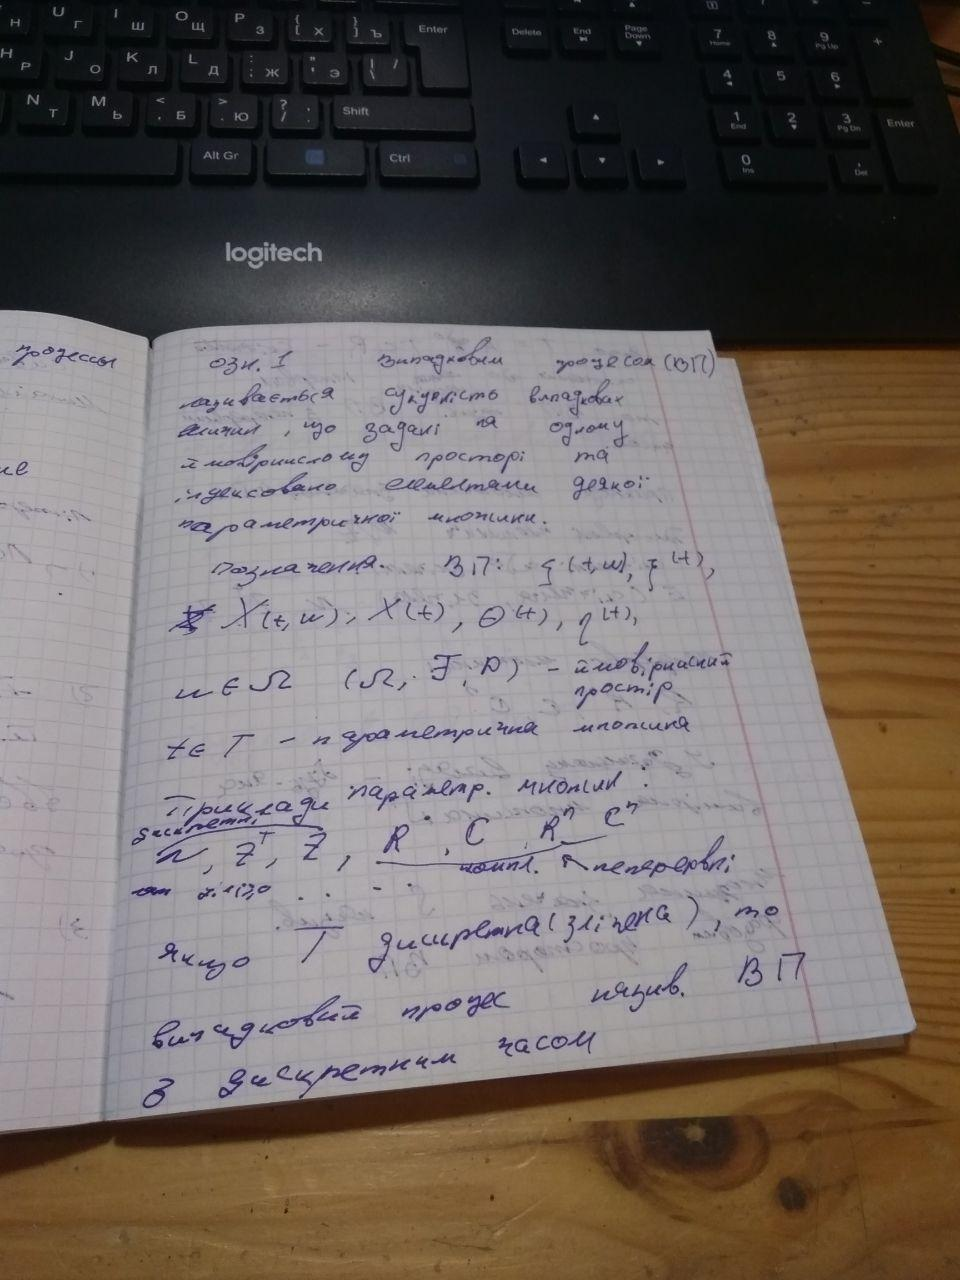
\includegraphics{{img/02/01}.png}
    \caption{Прямокутна скінченно-різницева сітка}
    \label{fig:2.1}
\end{figure}

Нижні індекси $i$ й $j$ ставляться до $x$ та $y$, а верхній індекс $n$ відповідає часовому шару. Кроки сітки в напрямках $i$ і $j$ позначаються через $\Delta x$ і $\Delta y$ відповідно. (Для простоти $\Delta x$ й $\Delta y$ вважаються постійними.) $f$ --- деяка функція. \medskip

Форми односторонніх різницевих виразів для першої похідної $\frac{\partial f}{\partial x}$ можна вивести в такий спосіб: припускаємо неперервність похідних і розкладаємо $f$ в ряд Тейлора в околі точки $(i, j)$. Верхній індекс (часовий) для простоти опускаємо. Тоді
\begin{equation}
    \label{eq:2.1}
    \begin{aligned}
        f_{i + 1, j} &= f_{i, j} + \left. \frac{\partial f}{\partial x} \right|_{i, j} (x_{i + 1, j} - x_{i, j}) + \frac{1}{2} \left. \frac{\partial^2 f}{\partial x^2} \right|_{i, j} (x_{i + 1, j} - x_{i, j})^2 + \ldots = \\
        &= f_{i, j} + \left. \frac{\partial f}{\partial x} \right|_{i, j} \Delta x + \frac{1}{2} \left. \frac{\partial^2 f}{\partial x^2} \right|_{i, j} \Delta x^2 + o(\Delta x^2).
    \end{aligned}
\end{equation}

Розв'язуючи це рівняння відносно $\frac{\partial f}{\partial x}$, одержуємо
\begin{equation*}
    \left. \frac{\partial f}{\partial x} \right|_{i, j} = \frac{f_{i + 1, j} - f_{i, j}}{\Delta x} - \frac{1}{2} \left. \frac{\partial^2 f}{\partial x^2} \right|_{i, j} \Delta x + o(\Delta x),
\end{equation*}
або
\begin{equation}
    \label{eq:2.2}
    \left. \frac{\partial f}{\partial x} \right|_{i, j} = \frac{f_{i + 1, j} - f_{i, j}}{\Delta x} + O(\Delta x),
\end{equation}

\begin{th_formula}[різницева апроксимація вперед]
    Позначимо скінченно-різницевий аналог $\frac{\partial f}{\partial x}$ через $\frac{\delta f}{\delta x}$. Тоді для $\frac{\delta f}{\delta x}$ при різницевій апроксимації вперед одержуємо вираз
    \begin{equation}
        \label{eq:2.3}
        \left. \frac{\delta f}{\delta x} \right|_{i, j} = \frac{f_{i + 1, j} - f_{i, j}}{\Delta x},
    \end{equation}
    з похибкою апроксимації порядку $\Delta x$, тобто з першим порядком точності. \medskip
\end{th_formula}

\begin{th_formula}[різницева апроксимація назад]
    Аналогічно, розкладаючи $f_{i - 1, j}$ в околі точки $(i, j)$, одержуємо для $\frac{\delta f}{\delta x}$ вираз при різницевій апроксимації назад:
    \begin{equation}
        \label{eq:2.4}
        \left. \frac{\delta f}{\delta x} \right|_{i, j} = \frac{f_{i, j} - f_{i - 1, j}}{\Delta x},
    \end{equation}
    який також має перший порядок точності. 
\end{th_formula}

Центральна (симетрична) різницева апроксимація $\frac{\delta f}{\delta x}$ виходить як різниця розкладів
\begin{equation}
    \label{eq:2.5}
    \begin{aligned}
        f_{i + 1, j} &= f_{i, j} + \left. \frac{\partial f}{\partial x} \right|_{i, j} \Delta x + \frac{1}{2} \left. \frac{\partial^2 f}{\partial x^2} \right|_{i, j} \Delta x^2 + \\ 
        &\quad + \frac{1}{6} \left. \frac{\partial^3 f}{\partial x^3} \right|_{i, j} \Delta x^3 + \frac{1}{24} \left. \frac{\partial^4 f}{\partial x^4} \right|_{i, j} \Delta x^4 + o(\Delta x^4).
    \end{aligned}
\end{equation}
та
\begin{equation}
    \label{eq:2.6}
    \begin{aligned}
        f_{i - 1, j} &= f_{i, j} - \left. \frac{\partial f}{\partial x} \right|_{i, j} \Delta x + \frac{1}{2} \left. \frac{\partial^2 f}{\partial x^2} \right|_{i, j} \Delta x^2 - \\ 
        &\quad - \frac{1}{6} \left. \frac{\partial^3 f}{\partial x^3} \right|_{i, j} \Delta x^3 + \frac{1}{24} \left. \frac{\partial^4 f}{\partial x^4} \right|_{i, j} \Delta x^4 - o(\Delta x^4).
    \end{aligned}
\end{equation}

Справді, віднімаючи \eqref{eq:2.6} від \eqref{eq:2.5}, одержуємо
\begin{equation*}
    f_{i + 1, j} - f_{i - 1, j} = 2 \left. \frac{\partial f}{\partial x} \right|_{i, j} \Delta x + \frac{1}{3} \left. \frac{\partial^3 f}{\partial x^3} \right|_{i, j} \Delta x^3 + o(x^4).
\end{equation*}

Розв'язуючи відносно $\frac{\partial f}{\partial x}$, маємо
\begin{equation}
    \label{eq:2.7}
    \begin{aligned}
        \left. \frac{\partial f}{\partial x} \right|_{i, j} &= \frac{f_{i + 1, j} - f_{i - 1, j}}{2\Delta x} - \frac{1}{6} \left. \frac{\partial^3 f}{\partial x^3} \right|_{i, j} \Delta x^2 + o(x^4) = \\
        &= \frac{f_{i + 1, j} - f_{i - 1, j}}{2\Delta x} + O(\Delta x^2).
    \end{aligned}
\end{equation}

\begin{th_formula}[центральна різницева апроксимація]
    Таким чином, центральна різницева апроксимація дає вираз
    \begin{equation}
        \label{eq:2.8}
        \left. \frac{\delta f}{\delta x} \right|_{i, j} = \frac{f_{i + 1, j} - f_{i - 1, j}}{2\Delta x}.
    \end{equation}
    з похибкою апроксимації порядку $\Delta x^2$, тобто із другим порядком точності.
\end{th_formula}

\begin{remark}
    Аналогічно можна одержати вирази для похідних по $y$ і $t$. Наприклад, центрально-різницевий аналог $\frac{\partial f}{\partial t}$ має вигляд
    \begin{equation}
        \label{eq:2.9}
        \left. \frac{\delta f}{\delta t} \right|_{i, j}^n = \frac{f_{i, j}^{n + 1} - f_{i, j}^{n - 1}}{2 \Delta t}.
    \end{equation}
\end{remark}

Виведемо тепер центрально-різницевий аналог $\frac{\partial^2 f}{\partial x^2}$. Додаючи \eqref{eq:2.5} і \eqref{eq:2.6}, маємо
\begin{equation}
    \label{eq:2.10}
    f_{i + 1, j} + f_{i - 1, j} = 2 f_{i, j} + \left. \frac{\partial^2 f}{\partial x^2} \right|_{i, j} \Delta x^2 + \frac{1}{12} \left. \frac{\partial^4 f}{\partial x^4} \right|_{i, j} \Delta x^4 + o(x^4).
\end{equation}

Розв'язуючи це рівняння відносно $\frac{\partial^2 f}{\partial x^2}$, одержуємо
\begin{equation}
    \label{eq:2.11}
    \left. \frac{\partial^2 f}{\partial x^2} \right|_{i, j} = \frac{f_{i + 1, j} - 2 f_{i, j} + f_{i - 1, j}}{\Delta x^2} + \frac{1}{12} \left. \frac{\partial^4 f}{\partial x^4} \right|_{i, j} \Delta x^2 + o(x^2).
\end{equation}

\begin{th_formula}[центральна різницева апроксимація другої похідної]
    Звідси для $\frac{\delta^2 f}{\delta x^2}$ маємо
    \begin{equation}
        \label{eq:2.12}
        \left. \frac{\delta^2 f}{\delta x^2} \right|_{i, j} = \frac{f_{i + 1, j} - 2 f_{i, j} + f_{i - 1, j}}{\Delta x^2}.
    \end{equation}
    із другим порядком точності.
\end{th_formula}

Також виконуються наступні формули:
\begin{equation}
    \label{eq:2.13}
    \left. \frac{\delta g}{\delta x} \right|_{i, j} = \frac{g_{i + 1/2, j} - g_{i - 1/2, j}}{\Delta x}
\end{equation}
та
\begin{equation}
    \label{eq:2.14}
    \left. \frac{\delta^2 f}{\delta x \delta y} \right|_{i, j} = \frac{f_{i + 1, j + 1} - f_{i + 1, j - 1} - f_{i - 1, j + 1} + f_{i - 1, j - 1}}{4 \Delta x \Delta y}.
\end{equation}
\begin{exercise}
    Доведіть ці формули.
\end{exercise}

\begin{remark}
    Мішана похідна $\frac{\partial^2 f}{\partial x \partial y}$ визначена формулою \eqref{eq:2.14} задовольняє відомій тотожності $\frac{\partial^2 f}{\partial x \partial y} = \frac{\partial^2 f}{\partial y \partial x}$ яка справджується для усіх двічі неперервно диференційовних функцій. Завжди бажано, щоб скінченно-різницеві рівняння добре моделювали якісну поведінку диференціальних рівнянь.
\end{remark}

Комбінації отриманих скінченно-різницевих виразів для частинних похідних можна використовувати для написання скінченно-різницевих формул диференціальних рівнянь у частинних похідних. Наприклад, рівняння Лапласа
\begin{equation*}
    \nabla^2 f = \frac{\partial^2 f}{\partial x^2} + \frac{\partial^2 f}{\partial y^2} = 0
\end{equation*}
буде мати різницевий аналог
\begin{equation*}
    \frac{\delta^2 f}{\delta x^2} + \frac{\delta^2 f}{\delta y^2} = \frac{f_{i + 1, j} - 2 f_{i, j} + f_{i - 1, j}}{\Delta x^2} + \frac{f_{i, j + 1} - 2 f_{i, j} + f_{i, j - 1}}{\Delta y^2} = 0,
\end{equation*}
або
\begin{equation}
    \label{eq:2.15}
    f_{i + 1, j} + f_{i - 1, j} - 2 (1 + \beta^2) f_{i, j} + \beta^2 (f_{i, j + 1} + f_{i, j - 1}) = 0,
\end{equation}
де $\beta$ --- відношення розмірів кроків, $\beta = \Delta x / \Delta y$. Це так званий п'ятиточковий аналог рівняння Лапласа. При $\beta = 1$ виходить відоме рівняння
\begin{equation}
    \label{eq:2.16}
    f_{i, j} = \frac{1}{4} \Big( f_{i + 1, j} + f_{i - 1, j} + f_{i, j + 1} + f_{i, j - 1} \Big),
\end{equation}
яке означає, що $f_{i, j}$ є середнім значенням $f$ у чотирьох сусідніх точках. Ці формули схематично зображені на наступному малюнку:
\begin{figure}[H]
    \centering
    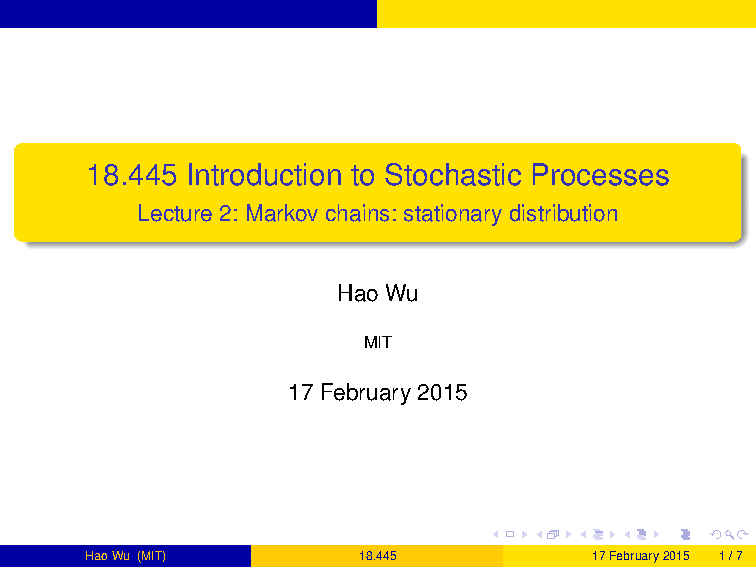
\includegraphics{{img/02/02}.png}
    \caption{Схематичне зображення п'ятиточкового аналога рівняння Лапласа}
    \label{fig:2.2}
\end{figure}

\begin{remark}
    Схема ліворуч відповідає довільному значенню $\beta$, праворуч --- $\beta = 1$.    
\end{remark}

Використовуючи для апроксимації просторових похідних і похідної за часом різницеві вирази другого порядку точності, лінійне модельне рівняння \eqref{eq:1.18} можна записати у вигляді
\begin{equation}
    \label{eq:2.17}
    \frac{\zeta_i^{n + 1} - \zeta_i^{n - 1}}{2 \Delta t} = - \frac{u \zeta_{i + 1}^n - u \zeta_{i - 1}^n}{2 \Delta x} + \alpha \frac{\zeta_{i + 1}^n - 2 \zeta_i^n + \zeta_{i - 1}^n}{\Delta x^2},
\end{equation}
що дозволяє явно виразити $\zeta_i^{n + 1}$ через значення змінних на попередніх часових шарах. Однак така схема в дійсності виявляється неприйнятною. Для всіх $\alpha > 0$ і всіх можливих $\Delta t > 0$ ця схема чисельно нестійка, тобто приводить до виникнення хаотичних розв'язків, що не мають відношення до істинного розв'язку диференціального рівняння. Така поведінка підкреслює відмінність між точними скінченно-різницевими аналогами для похідних і точним аналогом диференціального рівняння. \medskip

Якщо замість центральних різниць у нестаціонарному члені використовувати різниці вперед за часом, то вийде різницевий аналог лінійного модельного рівняння, що має другий порядок точності по просторовій змінній і лише перший за часом
\begin{equation}
    \label{eq:2.18}
    \frac{\zeta_i^{n + 1} - \zeta_i^n}{\Delta t} = - \frac{u \zeta_{i + 1}^n - u \zeta_{i - 1}^n}{2 \Delta x} + \alpha \frac{\zeta_{i + 1}^n - 2 \zeta_i^n + \zeta_{i - 1}^n}{\Delta x^2},
\end{equation}

\begin{definition}
    Цю схему з однобічними різницями вперед за часом і центральними (симетричними) різницями по просторовій змінній іноді називають схемою FTCS (від \textit{eng.} Forward-Time Central-Space).
\end{definition}

Надалі буде показано, що ця схема стійка (принаймні при деяких умовах, накладених на $\Delta t$, $u$, $\alpha$ і $\Delta x$). Але перш ніж приступити до дослідження стійкості, розглянемо деякі інші питання, пов'язані з скінченно-різницевими рівняннями.

\subsubsection{Поліноміальна апроксимація}

Інший метод одержання скінченно-різницевих виразів заснований на застосуванні апроксимуючої аналітичної функції з вільними параметрами, яка будується за значеннями у вузлах сітки й потім аналітично диференціюється. Це звичайний метод знаходження похідних за експериментальним даними. В ідеалі вигляд апроксимуючої функції повинен визначатися наближеним аналітичним розв'язком, однак звичайно в якості апроксимуючих функцій використовуються поліноми. Ми продемонструємо даний метод на прикладі параболічної апроксимації. \medskip

Припустимо, що значення функції $f$ задані в точках $i - 1$, $i$ та $i + 1$, і проведемо параболічну апроксимацію функції:
\begin{equation}
    \label{eq:2.19}
    f(x) = a + b x + c x^2,
\end{equation}
причому для зручності за початок координат ($x = 0$) приймемо точку $i$. Тоді рівняння \eqref{eq:2.19}, записане в точках $i - 1$, $i$ та $i + 1$ відповідно, дасть
\begin{equation}
    \label{eq:2.20}
    f_{i - 1} = a - b \Delta x + c \Delta x^2, \quad f_i = a, \quad f_{i + 1} = a + b \Delta x + c \Delta x^2. 
\end{equation}

Додаючи першу та третю рівності, одержуємо
\begin{equation}
    \label{eq:2.21}
    c = \frac{f_{i + 1} - 2 f_i + f_{i - 1}}{2 \Delta x^2}, 
\end{equation}
а розв'язуючи їх відносно $b$, знаходимо
\begin{equation}
    \label{eq:2.22}
    c = \frac{f_{i + 1} - f_{i - 1}}{2 \Delta x}.
\end{equation}

У точці $i$ значення першої похідної \eqref{eq:2.19} буде
\begin{equation}
    \label{eq:2.23}
    \left. \frac{\delta f}{\delta x} \right|_i = [b + 2 c x]_{x = 0} = b,
\end{equation}
а значення другої похідної
\begin{equation}
    \label{eq:2.24}
    \left. \frac{\delta^2 f}{\delta x^2} \right|_i = 2 c.
\end{equation}

Формули \eqref{eq:2.23} і \eqref{eq:2.24} з врахуванням \eqref{eq:2.21} і \eqref{eq:2.22} у точності збігаються з формулами \eqref{eq:2.8} і \eqref{eq:2.12} другого порядку із центральними різницями, отриманими розкладанням у ряд Тейлора. Якщо припустити, що $f$ --- поліном першого ступеня, тобто $f = a + bx$, то залежно від того, які значення використовуються для визначення $a$ й $b$: значення $f_i$ й $f_{i + 1}$ або $f_i$ й $f_{i - 1}$ для $\frac{\delta f}{\delta x}$ виходять формули з різницями вперед або назад відповідно. Очевидно, що при лінійній апроксимації $f$ не можна одержати вирази для $\frac{\delta^2 f}{\delta x^2}$. Однак якщо використовувати поліном першого ступеня для побудови різницевих аналогів перших похідних $\left. \frac{\delta f}{\delta x} \right|_{i + 1/2}$ і $\left. \frac{\delta f}{\delta x} \right|_{i - 1/2}$, які відповідно представляються різницями вперед та назад, то для $\frac{\delta^2 f}{\delta x^2}$ вийде вираз, що збігається з виразом \eqref{eq:2.12} із центральними різницями. \medskip

Різницеві формули для похідних більш високого порядку виводяться з використанням поліномів вищих порядків. Вирази, отримані за допомогою поліномів порядків вище другого, вже не ідентичні виразам, отриманим розкладаннями в ряди Тейлора, і в кожному випадку похибка апроксимації повинна перевірятися за допомогою розкладання в ряд Тейлора. В обчислювальній гідродинаміці метод поліноміальної апроксимації, як правило, застосовується тільки для обчислень значень похідних поблизу границь.\medskip

Тепер відзначимо недоліки поліноміальних апроксимацій вищого порядку, добре відомі фахівцям, що обробляють дані вимірів. Зі збільшенням порядку апроксимації вони стають чутливими до ``шумів'', тобто до більш-менш випадково розподілених малих помилок у даних.
\begin{example}
    Так, поліном шостого ступеня, графік якого проходить через сім точок, точно розташованих на одній прямій, приводить до апроксимації у вигляді прямої, зображеної на мал.~\ref{fig:2.3}.а. Однак при додаванні до значень, що апроксимуються, шумових збурювань коефіцієнти полінома будуть уже визначатися цими перекрученими даними, і тоді аналітичне обчислення похідних у точці $i$ може привести до абсурдних результатів, що можна побачити на мал.~\ref{fig:2.3}.б:
    \begin{figure}[H]
        \centering
        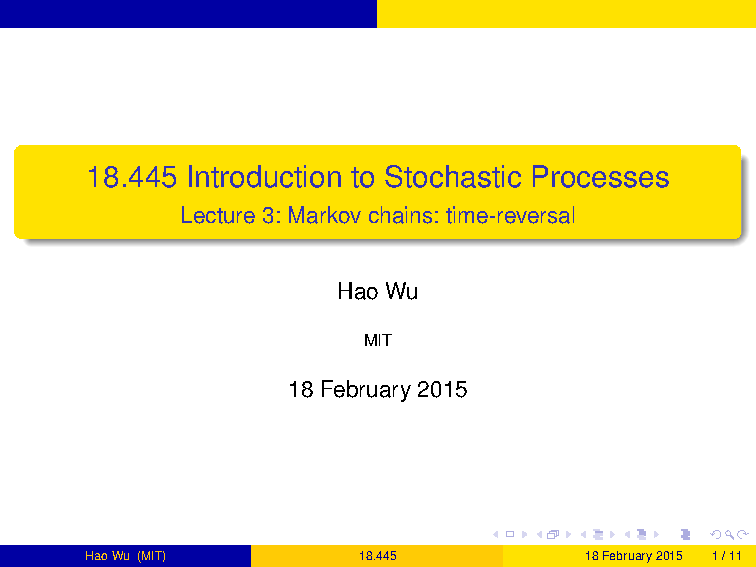
\includegraphics{{img/02/03}.png}
        \caption{Поліноміальна апроксимація шостого порядку}
        \label{fig:2.3}
    \end{figure}
\end{example}

\begin{remark}
    Квадратична апроксимація не може відобразити наявність точки перегину в розглянутих даних, тобто точки, де $\frac{\partial^2 f}{\partial x^2}$. Із цієї причини для аналізу наявних даних може бути виправдане використання поліноміальних апроксимацій третього порядку. (Часто використовуються сплайн-функції, що гарантують неперервність похідних при переході від однієї вузлової точки до іншої.) У нашому випадку рівняння, що описують розглянуте фізичне явище, не залежать від наявності точки перегину або від третьої похідної, тому немає необхідності зупинятися на цьому питанні.
\end{remark}

\subsubsection{Інтегральний метод}

В інтегральному методі потрібно приблизно задовольнити основним рівнянням, записаним в інтегральній, а не в диференціальній формі. Тут зручніше використовувати для просторової координати нижній індекс $x$, а для часу верхній індекс $t$ замість $i$ та $n$ відповідно. Запишемо лінійне модельне рівняння в консервативній формі:
\begin{equation}
    \label{eq:2.25}
    \frac{\partial \zeta}{\partial t} = - \frac{\partial (u \zeta)}{\partial x} + \alpha \frac{\partial^2 \zeta}{\partial x^2}
\end{equation}

Проінтегруємо це рівняння за часом від $t$ до $t + \Delta t$ і по просторовій області $R$ від $x - \Delta x / 2$ до $x + \Delta x / 2$, як показано на малюнку:
\begin{figure}[H]
    \centering
    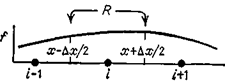
\includegraphics{{img/02/04}.png}
    \caption{Область інтегрування $R$ для інтегрального методу.}
    \label{fig:2.4}
\end{figure}

Оскільки порядок інтегрування по $t$ і $x$ неістотний (теорема Фубіні), виберемо його так, щоб можна було провести одне точне інтегрування, а саме
\begin{multline}
    \label{eq:2.26}
    \int_{x - \Delta x/2}^{x + \Delta x / 2} \left[ \int_t^{t + \Delta t} \frac{\partial \xi}{\partial t} \diff t \right] \diff x = - \int_t^{t + \Delta t} \left[ \int_{x - \Delta x/2}^{x + \Delta x / 2} \frac{\partial (u \zeta)}{\partial x} \diff x \right] \diff t + \\ + \alpha \int_t^{t + \Delta t} \left[ \int_{x - \Delta x/2}^{x + \Delta x / 2} \frac{\partial^2 \zeta}{\partial x^2} \diff x \right] \diff t.
\end{multline}

Виконаємо інтегрування виразів, записаних у квадратних дужках:
\begin{multline}
    \label{eq:2.27}
    \int_{x - \Delta x/2}^{x + \Delta x / 2} [ \zeta^{t + \Delta t} - \zeta^t] \diff x = - \int_t^{t + \Delta t} [ (u \zeta)_{x + \Delta x / 2} - (u \zeta)_{x - \Delta x / 2}] \diff t + \\ + \alpha \int_t^{t + \Delta t} \left[ \left. \frac{\partial \zeta}{\partial x} \right|_{x + \Delta x / 2} - \left. \frac{\partial \zeta}{\partial x} \right|_{x - \Delta x / 2} \right] \diff t.
\end{multline}

Інтеграли, що залишилися, визначимо чисельно. За теоремою про середнє можна записати
\begin{equation*}
    \int_{z_1}^{z_1 + \Delta z} f(z) \diff z \approx f(\bar z) \Delta z,
\end{equation*}
де $\bar z \in [z_1, z_1 + \Delta z]$. Збіжність гарантується при $\Delta z \to 0$. Взявши при наближеному обчисленні інтегралів у лівій частині рівняння \eqref{eq:2.27} середню точку $x$, а в правій частині значення підінтегральних функцій при нижній межі, тобто при $t$ (формула прямокутників), одержимо
\begin{multline}
    \label{eq:2.28}
    \left[ \zeta_x^{t + \Delta t} - \zeta_x^t \right] \Delta x = - \left[ (u \zeta)_{x + \Delta x / 2}^t - (u \zeta)_{x - \Delta x / 2}^t\right] \Delta t + \\ + \alpha \left[ \left. \frac{\partial \zeta}{\partial x} \right|_{x + \Delta x / 2}^t - \left. \frac{\partial \zeta}{\partial x} \right|_{x - \Delta x / 2}^t \right] \Delta t.
\end{multline}

Похідні $\frac{\partial \zeta}{\partial x}$ можна знайти зі співвідношення
\begin{equation*}
    \zeta_{x + \Delta x}^t = \zeta_x^t + \int_x^{x + \Delta x} \left. \frac{\partial \zeta}{\partial x} \right|^t \diff x.
\end{equation*}

Звідси використовуючи теорему про середнє, одержуємо
\begin{equation*}
    \zeta_{x + \Delta x}^t = \zeta_x^t + \left. \frac{\partial \zeta}{\partial x} \right|_{x + \Delta x/2}^t \Delta x.
\end{equation*}
або
\begin{equation}
    \label{eq:2.29}
    \left. \frac{\partial \zeta}{\partial x} \right|_{x + \Delta x/2}^t = \frac{\zeta_{x + \Delta x}^t - \zeta_x^t}{\Delta x}.
\end{equation}

Значення $(u \zeta)_{x + \Delta x / 2}^t$ можна обчислити як середнє арифметичне:
\begin{equation}
    \label{eq:2.30}
    (u \zeta)_{x + \Delta x / 2}^t = \frac{1}{2} \Big( (u \zeta)_x^t + (u \zeta)_{x + \Delta x}^t \Big).
\end{equation}

Аналогічний вираз має місце й для $(u \zeta)_{x - \Delta x / 2}^t$. \medskip

Підставляючи \eqref{eq:2.29} і \eqref{eq:2.30} в \eqref{eq:2.28}, знаходимо
\begin{multline*}
    \left[ \zeta_x^{t + \Delta t} - \zeta_x^t \right] \Delta x = - \left[ \frac{1}{2} (u \zeta)_x^t + \frac{1}{2} (u \zeta)_{x + \Delta x}^t - \frac{1}{2} (u \zeta)_x^t - \frac{1}{2} (u \zeta)_{x - \Delta x}^t \right] \Delta t + \\ + \alpha \left[ \frac{\zeta_{x + \Delta x}^t - \zeta_x^t}{\Delta x} - \frac{\zeta_x^t - \zeta_{x - \Delta x}^t}{\Delta x} \right] \Delta t.
\end{multline*}

Розділивши останнє рівняння на $\Delta x \Delta t$, одержимо
\begin{equation}
    \label{eq:2.31}
    \frac{\zeta_x^{t + \Delta t} - \zeta_x^t}{\Delta t} = - \frac{(u \zeta)_{x + \Delta x}^t - (u \zeta)_{x - \Delta x}^t}{2\Delta x} + \alpha \frac{\zeta_{x + \Delta x}^t - 2 \zeta_x^t + \zeta_{x - \Delta x}^t}{\Delta x^2}.
\end{equation}

Переходячи до індексів $i$ та $n$, бачимо, що рівняння \eqref{eq:2.31} співпадає з рівнянням \eqref{eq:2.18}, виведеним за допомогою розкладань у ряди Тейлора. 

\begin{remark}
    У будь-якому методі існує велика довільність при виводі скінченно-різницевих рівнянь. 
\end{remark}

\begin{example}
    Якщо інтегрувати за часом не від $t$ до $t + \Delta t$, а від $t - \Delta t$ до $\Delta t$, а в якості середньої точки обрати $t$, то вийде рівняння \eqref{eq:2.17}. (Як уже було відзначено вище, це рівняння безумовне нестійке.)
\end{example}

\begin{remark}
    Переваги інтегрального методу можна буде оцінити після того, як буде вивчена властивість консервативності. Відмінність між інтегральним методом і методом розкладання в ряди Тейлора найбільш чітко проявляється при використанні непрямокутних систем координат.
\end{remark}

\subsubsection{Метод контрольного об'єму}

Метод контрольного об'єму для виводу скінченно-різницевих рівнянь дуже схожий на інтегральний метод, але більш фізичний по суті. Цей метод найбільше яскраво висвітлює процес ``чисельного моделювання''. Найкращими прикладами такого підходу можуть служити широко відомий метод часток у гніздах (\textit{eng.} PIC) і метод рідини в гніздах (\textit{eng.} FLIC), розвинені в Лос-Аламосскій лабораторії (Еванс і Харлоу [1947]; Джентрі, Мартін і Далі [1966]). \medskip

Виберемо в просторі контрольний об'єм із центром у точці $x$, як показано на малюнку:
\begin{figure}[H]
    \centering
    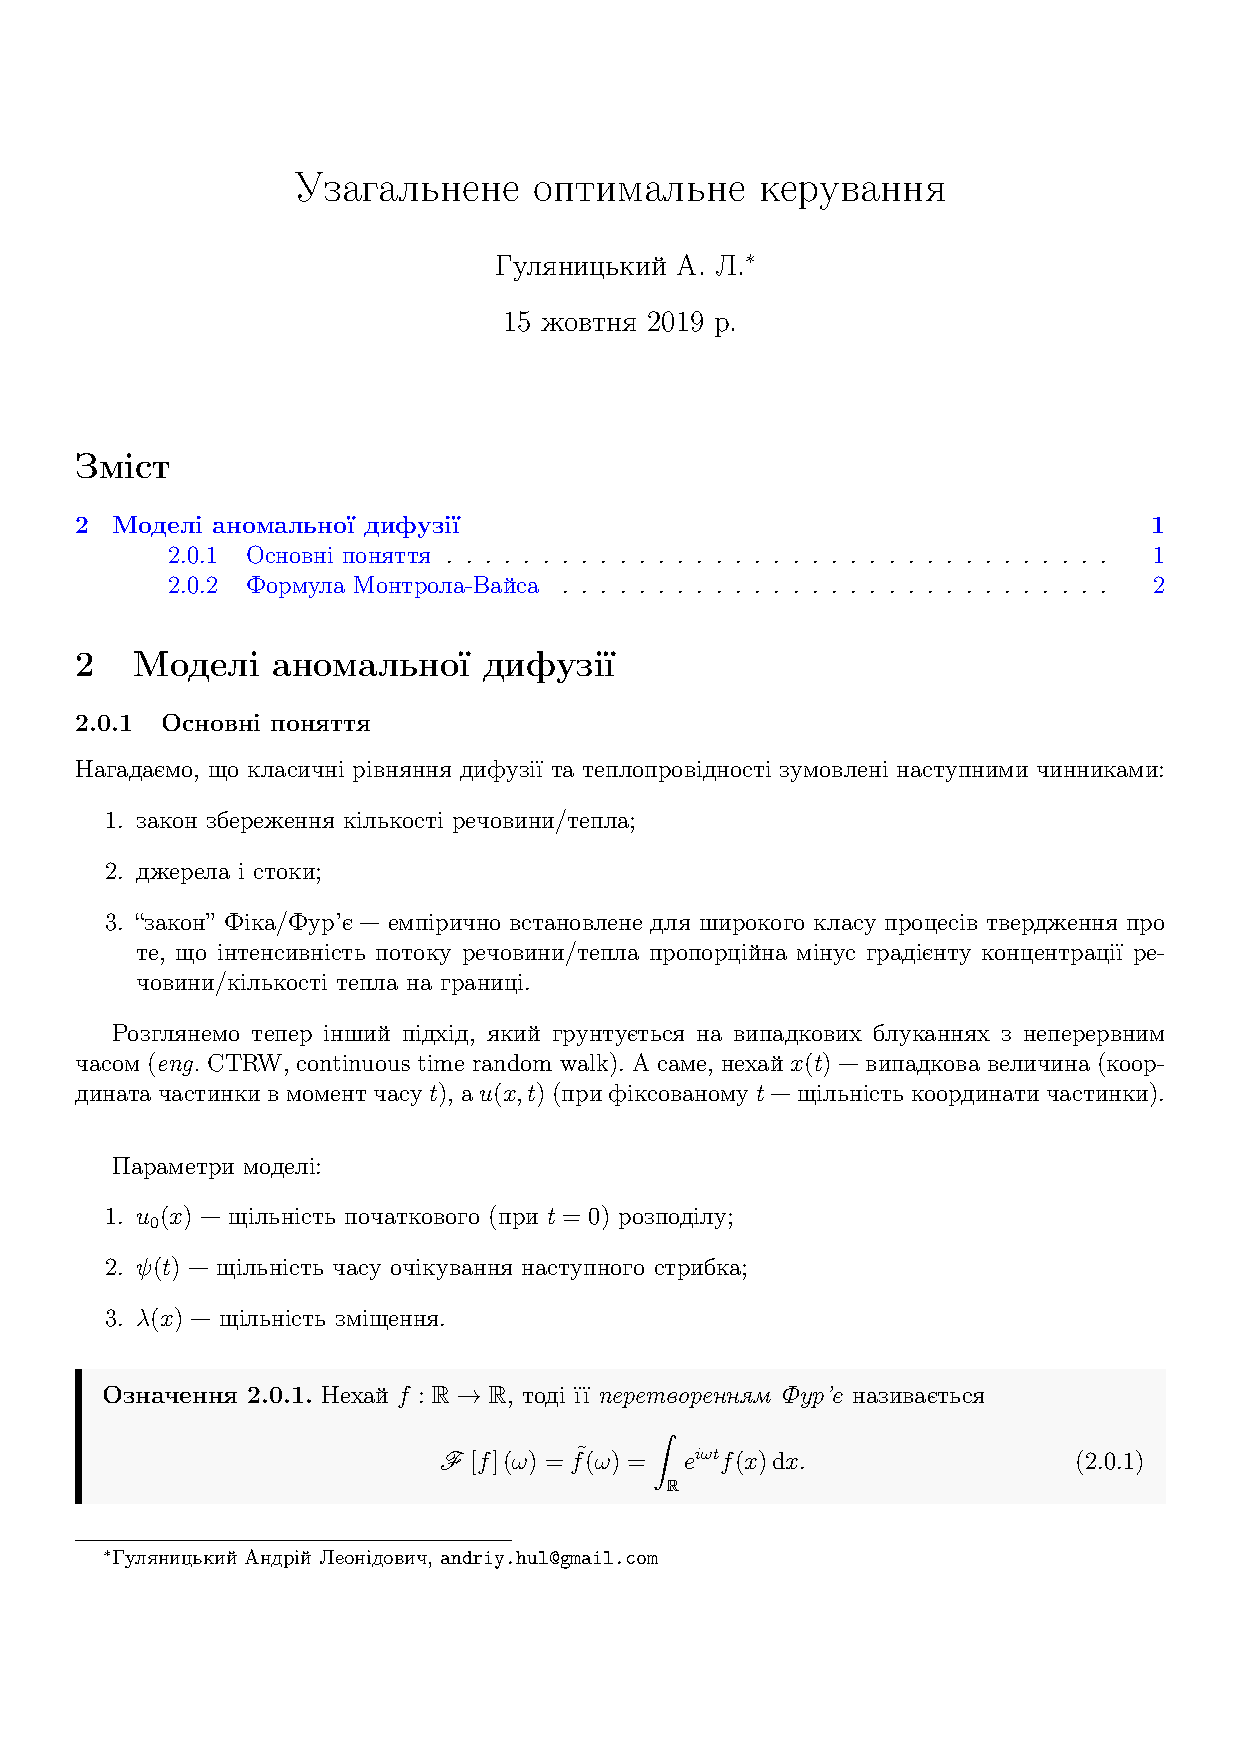
\includegraphics{{img/02/05}.png}
    \caption{Контрольний об'єм (КО) в точці $x$}
    \label{fig:2.5}
\end{figure}

У якості значення $\zeta$ у вузловій точці сітки будемо брати середнє значення цієї функції по контрольному об'єму (КО). Для питомої (тобто усередненої за об'ємом) величини $\zeta$, де $\zeta$ можна тепер розглядати як будь-яку змінну величину, запишемо $\zeta = \Gamma\text{/об'єм}$. \medskip

Наприклад, якщо $\zeta$ --- щільність $\rho$, то $\Gamma$ --- повна маса, укладена в розглянутому контрольному обсязі із центром у точці $x$. Якщо $\zeta$ --- вихор, то $\Gamma$ --- циркуляція. Тепер запишемо словесне формулювання наступного закону збереження:

\begin{th_law}
    \label{law:control-space}
    Повне збільшення величини $\Gamma$ у КО $=$ чистий приплив $\Gamma$ у КО за рахунок конвекції $+$ чистий приплив $\Gamma$ у КО за рахунок дифузії.
\end{th_law}
    
Повне збільшення величини $\Gamma$ $=$ $\xi$ $\times$ (об'єм) у КО за проміжок часу $\Delta t$ рівно
\begin{equation*}
    \left. \zeta \right|_x^{t + \Delta t} \times (\Delta x \Delta y \Delta z) - \left. \zeta \right|_x^t \times (\Delta x \Delta y \Delta z).
\end{equation*}

Конвективний потік величини $\Gamma$, що втікає в КО через ліву грань за одиницю часу, становить
\begin{equation*}
    (u \zeta)_{x - \Delta x / 2} \times (\text{площа лівої грані}) = (u \zeta)_{x - \Delta x / 2} \times (\Delta y \Delta z),
\end{equation*}
де $u$ може бути змінною, а значення функцій на грані $x - \Delta x / 2$, які ще треба визначити, повинні бути деякими середніми за $\Delta t$. Виходячи із цієї величини вхідного конвективного потоку за одиницю часу, повний конвективний потік величини $\Gamma$ у КО за проміжок часу $\Delta t$ через грань $x - \Delta x / 2$  можна записати так:
\begin{equation*}
    (u \zeta)_{x - \Delta x / 2} \Delta y \Delta z \Delta t.
\end{equation*}

Аналогічно, повний конвективний потік $\Gamma$, що виходить з КО через $x + \Delta x / 2$, буде рівний
\begin{equation*}
    (u \zeta)_{x + \Delta x / 2} \Delta y \Delta z \Delta t,
\end{equation*}
а чистий приріст $\Gamma$ у КО виходить як різниця сумарного потоку, що втікає, і сумарного потоку, що витікає, тобто
\begin{equation*}
    \Big[ (u \zeta)_{x - \Delta x / 2} - (u \zeta)_{x + \Delta x / 2} \Big] \Delta y \Delta z \Delta t.
\end{equation*}

Щоб обчислити потік у КО за рахунок дифузії, необхідно мати закон для швидкості дифузії. Найпростіший такий закон (що узгодиться з рівнянням переносу вихору) є лінійним і говорить, що дифузійний потік величини $\zeta$ за одиницю часу, який ми назвемо $q$, пропорційний градієнту $\zeta$ (закон Фіка):
\begin{equation*}
    q = - \alpha \frac{\partial \zeta}{\partial x}.
\end{equation*}

Тут мінус указує на те, що збільшення $\zeta$ в напрямку $x$ викликає дифузію в протилежному напрямку. \medskip

Дифузійний потік, що втікає в КО через ліву грань за одиницю часу, рівний
\begin{equation*}
    \left. q \right|_{x - \Delta x / 2} \Delta y \Delta z = - \alpha \left. \frac{\partial \zeta}{\partial x} \right|_{x - \Delta x / 2} \Delta y \Delta z,
\end{equation*}
а потік, що випливає з КО через праву грань за одиницю часу становить
\begin{equation*}
    \left. q \right|_{x + \Delta x / 2} \Delta y \Delta z = - \alpha \left. \frac{\partial \zeta}{\partial x} \right|_{x + \Delta x / 2} \Delta y \Delta z,
\end{equation*}
 
Тут знову значення на гранях $x + \pm \Delta x / 2$ становить собою деякі середні за час $\Delta t$, які ще повинні бути визначені. Величина потоку в КО за рахунок дифузії за проміжок часу $\Delta t$ рівна
\begin{equation*}
    \alpha \Delta y \Delta z \Delta t \left[ \left. \frac{\partial \zeta}{\partial x} \right|_{x + \Delta x / 2} - \left. \frac{\partial \zeta}{\partial x} \right|_{x - \Delta x / 2} \right].
\end{equation*}
 
Тоді закон \ref{law:control-space} можна переписати наступни чином:
\begin{multline}
    \label{eq:2.32}
    \left. \zeta \right|_x^{t + \Delta t} \Delta x \Delta y \Delta z - \left. \zeta \right|_x^t \Delta x \Delta y \Delta z = \Big[ (u \zeta)_{x - \Delta x / 2} - (u \zeta)_{x + \Delta x / 2} \Big] \Delta y \Delta z \Delta t + \\ + \alpha \Delta y \Delta z \Delta t \left[ \left. \frac{\partial \zeta}{\partial x} \right|_{x + \Delta x / 2} - \left. \frac{\partial \zeta}{\partial x} \right|_{x - \Delta x / 2} \right].
\end{multline}

Розділивши на $\Delta x \Delta y \Delta z \Delta t$, одержимо
\begin{multline}
    \label{eq:2.33}
    \frac{1}{\Delta t} \left[ \left. \zeta \right|_x^{t + \Delta t} - \left. \zeta \right|_x^t \right] = \frac{1}{\Delta x} \Big[ (u \zeta)_{x - \Delta x / 2} - (u \zeta)_{x + \Delta x / 2} \Big] + \\ + \frac{\alpha}{\Delta x} \left[ \left. \frac{\partial \zeta}{\partial x} \right|_{x + \Delta x / 2} - \left. \frac{\partial \zeta}{\partial x} \right|_{x - \Delta x / 2} \right].
\end{multline}

Як і в інтегральному методі, при подальшому виводі скінченно-різницевих виразів з'являється деяка свобода дій при визначенні значень функцій на границях об'єму. У якості значень на границі об'єму можна обрати середнє арифметичне значення в сусідніх вузлах у момент часу $n$; тоді
\begin{equation*}
    (u \zeta)_{x \pm \Delta x} = \frac{1}{2} \Big[ (u \zeta)_{x \pm \Delta x}^n + (u \zeta)_x^n \Big]
\end{equation*}
і градієнти
\begin{equation*}
    \left. \frac{\partial \zeta}{\partial x} \right|_{x \pm \Delta x / 2} = \left. \frac{\delta \zeta}{\delta x} \right|_{x \pm \Delta x / 2}^n
\end{equation*}
можна обчислити за допомогою центральних різниць:
\begin{equation*}
    \left. \frac{\delta \zeta}{\delta x} \right|_{x \pm \Delta x / 2}^n = \frac{\left. \zeta \right|_{x \pm \Delta x}^n - \left. \zeta \right|_x^n}{\Delta x}.
\end{equation*}
 
У результаті рівняння \eqref{eq:2.33} набуде вигляду
\begin{multline}
    \label{eq:2.34}
    \frac{1}{\Delta t} \left[ \left. \zeta \right|_x^{t + \Delta t} - \left. \zeta \right|_x^t \right] = \frac{1}{\Delta x} \Bigg( \frac{1}{2} \Big[ (u \zeta)_{x + \Delta x}^n + (u \zeta)_x^n \Big] - \frac{1}{2} \Big[ (u \zeta)_{x - \Delta x}^n + (u \zeta)_x^n \Big] \Bigg) + \\ + \frac{\alpha}{\Delta x} \left[ \frac{\left. \zeta \right|_{x + \Delta x}^n - \left. \zeta \right|_x^n}{\Delta x} - \frac{\left. \zeta \right|_{x - \Delta x}^n - \left. \zeta \right|_x^n}{\Delta x} \right].
\end{multline}
або
\begin{equation}
    \label{eq:2.35}
    \frac{\zeta_x^{t + \Delta t} - \zeta_x^t}{\Delta t} = \frac{(u \zeta)_{x + \Delta x}^n - (u \zeta)_{x - \Delta x}^n}{2\Delta x} + \alpha \frac{\zeta_{x + \Delta x}^t - 2 \zeta_x^t + \zeta_{x - \Delta x}^t}{\Delta x^2}.
\end{equation}

Якщо повернутися до індексів $i$ та $n$, то це рівняння збіжиться з отриманим раніше рівнянням \eqref{eq:2.18}. \medskip

У такий спосіб видно, що всі чотири методи виводу скінченно-різницевих аналогів диференціальних рівнянь у частинних похідних --- розкладання в ряд Тейлора, метод поліноміальної апроксимації, інтегральний метод і метод контрольного об'єму --- можуть привести до однакових різницевих виразів. Це обнадіює й зміцнює довіру до всіх цих методів. Але в кожному з них є деяка свобода дій, так що вибір методу для виводу скінченно-різницевого аналога диференціального рівняння визначає цей аналог не єдиним способом. Насправді, існує багато аналогів. Незважаючи на те що більшість із них різниться у незначних деталях, вони можуть сильно відрізнятися по своїй поведінці. Одним з дивних аспектів обчислювальної гідродинаміки є наявність великої кількості правдоподібних схем, які, однак, не працюють, як, наприклад, було зазначено для рівняння \eqref{eq:2.17}. Це справедливо як для основних (тобто призначених для розрахунків внутрішніх точок) різницевих схем, так і для схем, призначених для розрахунків граничних точок. \medskip

Перевага цього методу полягає в тому, що він заснований на макроскопічних фізичних законах, а не на використанні математичного апарата неперервних функцій. Особливо важливим це виявляється в тих випадках, коли мають справу з розрідженими газами або із динамікою нев'язкого газу з ударними хвилями. У цих випадках диференціальні рівняння не мають усюди неперервних розв'язків, які можна було б у кожній крапці представити рядами Тейлора. Однак маса, наприклад, все-таки зберігається, і конвективна частина рівняння \eqref{eq:2.35} як і раніше залишається справедливою. Але навіть і в тих випадках, коли неперервні розв'язки існують, у методі контрольного об'єму увага зосереджується на фактичному виконанні фізичних законів макроскопічно, а не тільки при $\Delta x$ і $\Delta t$, що прямують до нуля. Це лежить в основі поняття консервативності скінченно-різницевого методу, до обговорення якого ми переходимо.

\subsection{Властивість консервативності} %[Роуч, стор.51-58]

\begin{definition}
    Скінченно-різницевий метод є \textit{консервативним}, якщо він забезпечує виконання певних інтегральних законів збереження, справедливих для вихідних диференціальних рівнянь.
\end{definition}

Розглянемо рівняння переносу вихору \eqref{eq:1.12}:
\begin{equation*}
    \frac{\partial \zeta}{\partial t} = - \nabla \cdot (V \zeta) + \frac{1}{\text{Re}} \nabla^2 \zeta,
\end{equation*}
поклавши $\frac{1}{\text{Re}} = \alpha$,
\begin{equation}
    \label{eq:2.36}
    \frac{\partial \zeta}{\partial t} = - \nabla \cdot (V \zeta) + \alpha \nabla^2 \zeta,
\end{equation}

Проінтегруємо це рівняння по деякій просторовій області $R$:
\begin{equation}
    \label{eq:2.37}
    \int_R \frac{\partial \zeta}{\partial t} \diff R = - \int_R \nabla \cdot (V \zeta) \diff R + \int_R \alpha \nabla^2 \zeta \diff R.
\end{equation}

Оскільки $t$ не залежить від просторових змінних, маємо
\begin{equation}
    \label{eq:2.38}
    \int_R \frac{\partial \zeta}{\partial t} \diff R = \frac{\partial}{\partial t} \int_R \zeta \diff R.
\end{equation}

Використовуючи формулу Гауса-Остроградського, одержуємо
\begin{equation}
    \label{eq:2.39}
    \int_R \nabla \cdot (V \zeta) \diff R = \int_{\partial R} (V \zeta) \cdot \vec n \diff s,
\end{equation}
де $\partial R$ --- границя $R$, $\vec n$ --- одиничний вектор нормалі до поверхні (додатний напрямок відповідає зовнішній нормалі) і $\diff s$ --- диференціал довжини дуги границі $\partial R$. Аналогічно, за тією ж формулою
\begin{equation}
    \label{eq:2.40}
    \int_R \alpha \nabla^2 \zeta \diff R = \alpha \int_{\partial R} (\nabla \zeta) \cdot \vec n \diff s,
\end{equation}

Тоді рівняння \eqref{eq:2.37} набуде вигляду
\begin{equation}
    \label{eq:2.41}
    \frac{\partial}{\partial t} \int_R \zeta \diff R = - \int_{\partial R} (V \zeta) \cdot \vec n \diff s + \alpha \int_{\partial R} (\nabla \zeta) \cdot \vec n \diff s.
\end{equation}

Це рівняння констатує, що швидкість накопичення величини $\zeta$ в області $R$ дорівнює сумі конвективного й дифузійного притоків величини $\zeta$ в $R$ через $\partial R$ за одиницю часу). 

\begin{definition}
    \textit{Вимога консервативності} полягає у тотожному збереженні у скінченно-різницевій схемі цього інтегрального співвідношення.
\end{definition}

Розглянемо одновимірне модельне рівняння для граничного випадку нев'язкої рідини ($\alpha = 0$), яке випливає з рівняння \eqref{eq:2.36} і має вигляд
\begin{equation}
    \label{eq:2.42}
    \frac{\partial \zeta}{\partial t} = - \frac{\partial (u \zeta)}{\partial x}.
\end{equation}

\begin{remark}
    Якщо величину $\zeta$ трактувати як масову густину, то рівняння \eqref{eq:2.42} буде рівнянням нерозривності для стисливого середовища.
\end{remark}

Використовуючи різниці вперед за часом і центральні різниці по просторовій змінної, можна записати скінченно-різницевий аналог рівняння \eqref{eq:2.42} у вигляді
\begin{equation*}
    \frac{\zeta_i^{n + 1} - \zeta_i^n}{\Delta t} = - \frac{u_{i + 1} \zeta_{i + 1} - u_{i - 1} \zeta_{i - 1}}{2 \Delta x}
\end{equation*}

\begin{remark}
    У правій частині тут і надалі опущено верхній індекс ${}^n$ оскільки він усюди однаковий.
\end{remark}

Розглянемо тепер одновимірну область $R$ (причому $i$ змінюється від $I_1$ до $I_2$) і обчислимо суму $\frac{1}{\Delta t} \sum_{i = I_1}^{I_2} \zeta_i \Delta x$, відповідну до інтеграла $\frac{\partial}{\partial t} \int_R \zeta \diff R$ в рівнянні \eqref{eq:2.41}:
\begin{align}
    \frac{1}{\Delta t} \left[ \sum_{i = I_1}^{I_2} \zeta_i^{n + 1} \Delta x - \sum_{i = I_1}^{I_2} \zeta_i^n \Delta x \right] &= \sum_{i = I_1}^{I_2} \left( - \frac{u_{i + 1} \zeta_{i + 1} - u_{i - 1} \zeta_{i - 1}}{2 \Delta x} \right) \Delta x = \nonumber \\
    \label{eq:2.43}
    &= \frac{1}{2} \sum_{i = I_1}^{I_2} [(u \zeta)_{i - 1} - (u \zeta)_{i + 1}] = \\
    &= \frac{1}{2} \Big( (u\zeta)_{I_1 - 1} + (u\zeta)_{I_1} \Big) - \frac{1}{2} \Big( (u\zeta)_{I_2} - (u\zeta)_{I_2 + 1} \Big) = \nonumber \\
    \label{eq:2.44}
    &= (u \zeta)_{I_1 - 1/2} - (u \zeta)_{I_2 + 1/2}.
\end{align}

\begin{remark}
    Сумування в \eqref{eq:2.43} відбулося за допомогою телескопічного методу.
\end{remark}
 
Отримане рівняння показує, що швидкість накопичення величини $\zeta$ в області $R$ в точності рівна потоку величини $\zeta$ в область $R$ через границі $I_1 - 1/2$ й $I_2 + 1/2$ (це випливає також з рівняння \eqref{eq:2.41} при $\alpha = 0$). Таким чином, отриманий скінченно-різницевий аналог зберігає інтегральну властивість, яку виражає формула Остроградського-Гауса для диференціального рівняння, і ми будемо говорити, що цей аналог має властивість консервативності. \medskip

Властивість консервативності залежить як від використаної форми диференціального рівняння, так і від прийнятої скінченно-різницевої схеми. 

\begin{example}
    Неконсервативна форма одновимірного модельного рівняння \eqref{eq:1.18} при $\alpha = 0$ така:
    \begin{equation}
        \label{eq:2.45}
        \frac{\partial \zeta}{\partial t} = - u \frac{\partial \zeta}{\partial x}.
    \end{equation}
\end{example}
\begin{proof}
    Використовуючи ту ж схему, що й у попередньому прикладі, тобто різниці вперед за часом і центральні різниці по просторовій змінної, одержуємо
    \begin{equation}
        \label{eq:2.46}
        \frac{\zeta_i^{n + 1} - \zeta_i^n}{\Delta t} = - u_i^n \frac{\zeta_{i + 1} - \zeta_{i - 1}}{2 \Delta x}.
    \end{equation}

    Тоді суми, що відповідають\eqref{eq:2.43}--\eqref{eq:2.44}, мають вигляд
    \begin{equation}
        \label{eq:2.47}
        \begin{aligned}
            \frac{1}{\Delta t} \left[ \sum_{i = I_1}^{I_2} \zeta_i^{n + 1} \Delta x - \sum_{i = I_1}^{I_2} \zeta_i^n \Delta x \right] &= \sum_{i = I_1}^{I_2} \left( - u_i \frac{\zeta_{i + 1} - \zeta_{i - 1}}{2 \Delta x} \right) \Delta x = \\
            &= \frac{1}{2} \sum_{i = I_1}^{I_2} u_i (\zeta_{i - 1} - \zeta_{i + 1}).
        \end{aligned}
    \end{equation}
    
    Але ця сума не може бути згорнута телескопічним методом! (за винятком частинного випадку, коли $u_i = \const$). Виходить, у цьому випадку скінченно-різницевий аналог виявляється не в змозі забезпечити виконання формули Остроградського-Гауса для диференціального рівняння. 
\end{proof}
\begin{remark}
    Тепер стає ясним зміст термінів ``консервативна'' і ``дивергентна'' форма рівняння \eqref{eq:1.10}.
\end{remark}

У першому випадку консервативність забезпечується застосуванням методу контрольного об'єму при виводі скінченно-різницевих виразів. При використанні консервативної форми конвективний потік величини $\zeta$, що випливає через грань $I_1 + 1/2$ із контрольного об'єму із центром у точці $i$ за одиницю часу, становить $(u_i\zeta_i+u_{i+1}\zeta_{i+1})/2$ і в точності рівний конвективному потоку, що втікає через ту ж грань у контрольний об'єм із центром у точці  за одиницю часу. Як показано вище, у випадку неконсервативної форми це не мало б місця.

\begin{exercise}
    Показати, що використання для $\frac{\partial^2 \zeta}{\partial x^2}$ виразу \eqref{eq:2.12} із центральними різницями при $\alpha > 0$ забезпечує консервативність для дифузійних членів.
\end{exercise}

Ясно, що при $\alpha > 0$ єдиний шлях забезпечити збереження сумарного потоку в загальному випадку (коли $u$ є функцією просторової змінної) полягає в незалежному збереженні конвективних і дифузійних членів; у неодновимірному випадку необхідно забезпечити консервативність цих членів окремо по кожної просторовій змінній. \medskip

Важливість властивості консервативності легко зрозуміти на прикладі рівняння нерозривності для стисливого середовища. Розглянемо задачу про природню конвекцію в повністю замкненому сосуді з непроникними стінками. У початковий момент часу вважаємо, що в повному обсязі $V = 0$. До нижньої стінки посудини підводить тепло, і відбувається природня конвекція, що можливо досягає стаціонарного стану. Якщо для розрахунків застосовується яка-небудь неконсервативна схема, то повна маса в досліджуваному об'ємі буде мінятися. Якщо ж використовується консервативна схема, то повна маса не буде мінятися (без врахування машинних помилок округлення). Слід зауважити, що помилки, викликані порушенням збереження маси, зменшуються при $\Delta x \to 0$, але в практичних обчисленнях зі скінченною величиною $\Delta x$ ці помилки є суттєвими. \medskip

Ці міркування ми вважаємо істотними й переконливо рекомендуємо застосовувати консервативні схеми. Однак тут є доводи й за й проти, причому приклади чисельних контрольних розрахунків, опубліковані в літературі, не дають можливості зробити однозначний вибір. Звернемося до цих доводів і до результатів контрольних розрахунків. \medskip

Властивість консервативності не обов'язково пов'язане з підвищенням точності схеми. Наприклад, нестійкі розв'язки консервативних рівнянь зберігають властивість консервативності. Більше того, неконсервативний метод може бути в деякому змісті точніше консервативного. Наприклад, для виразу функцій за значеннями у вузлах сітки можна було б застосовувати одновимірні апроксимації поліномами високого порядку й при цьому похідні по просторових змінних будуть, імовірно, визначатися з помилкою більш високого. Однак побудована в такий спосіб схема може бути неконсервативною, а якщо критерій точності включає умова консервативності, то неконсервативна схема виявиться менш точною. \medskip

Дотепер досвід показує, що консервативні схеми, загалом кажучи, дають більш точні результати. Чен [1968] і Аллен [1968] показали, що за допомогою консервативної схеми виходять суттєво більш точні результати для деяких розв'язків рівняння Бюргерса \eqref{eq:1.19} і \eqref{eq:1.20}. Сайрус і Фолтон [1967] з'ясували, що для еліптичних рівнянь консервативна схема дає більш точні результати, ніж неконсервативна. На прикладі задачі про плин усередині замкненої прямокутної області з однієї рухливою границею Торранс зі співавторами [1972] переконалися в тому, що навіть схема першого порядку точності для рівнянь у консервативній формі дає більш точні результати, ніж схема другого порядку для рівнянь у неконсервативній формі. Переваги розрахунків ударних хвиль при консервативній формі рівнянь (Ґері [1964]) добре відомі, однак слід помітити, що в роботі Гару хвилі розрідження трохи точніше розраховувалися за неконсервативною схемою. Крім того, дивергентна форма рівнянь більш осмислена фізично й полегшує постановку граничних умов для плинів стисливої рідини. \medskip

Піачек [1966] показав, як вивести консервативні рівняння в осесимметричном випадку. Робертс і Вейс [1966] обговорювали консервативність для векторних величин. Лаку [1954] першим використовував у скінченно-різницевих обчисленнях консервативну форму рівнянь руху стисливого газу, запропоновану Курантом і Фрідріхсом [1948], і детально досліджував властивість консервативності. \medskip

Метеорологи поширили ідею консервативності на величини, пов'язані з кількістю руху. Браян [1963, 1966] запропонував схеми, що забезпечують збереження не тільки вихру, але й кінетичної енергії. Схема Аракави [1966] зберігає вихор, квадрат вихру, кількість руху й кінетичну енергію. Але такі додаткові ускладнення схем не завжди виправдані й вигідні. Бенґтсон [1964] показав, що подібні ускладнені схеми дають невеликі поліпшення, незначні стосовно дійсних даних, і в той же час можуть привести до більших помилок у швидкості хвиль. Однак у граничному нев'язкому випадку збереження кінетичної енергії дає можливість уникнути ``нелінійної'' нестійкості, розглянутої в роботах Філіпса [1959] і Сандквіста [1963]. Бенґтсон [1964] запропонував схему, що зберігає різницю між кінетичною енергією й (метеорологічної) повною статичною стійкістю, що корисно в задачах з більшими градієнтами сили тяжіння. \medskip

Звичайно схеми, що забезпечують збереження основних величин, таких, як вихор, маса, кількість руху або повна енергія, не вимагають великої роботи. У двовимірній задачі про перенос вихру додаткова робота полягає у виконанні двох зайвих скінченно-різницевих операцій для одержання складових швидкості з розв'язку для функції струму й двох зайвих множень. У задачах про рух стисливого середовища додаткової роботи більше, що в деяких випадках може виявитися причиною відмови від застосування консервативної схеми (метод Моретті). При розв'язку багатьох задач консервативні схеми не використовувалися, див., наприклад, роботи Аллена й Саусвела [1955], Хина й Макано [1966], Позначка й Лавана [1968], Бао й Доґерті [1969]. Помітимо, що всі схеми методу характеристик є неконсервативними й що при скінченно-різницевому розв'язку рівнянь прикордонного шару консервативна схема звичайно також не використовується. У таких випадках властивість консервативності може служити для перевірки точності обчислень. \medskip

Помітимо на закінчення, що неконсервативна форма для члена $\frac{\partial}{\partial x} \left( \alpha \frac{\partial \zeta}{\partial x} \right)$ зі змінним коефіцієнтом дифузії може привести до більш точних результатів, ніж консервативна (див. задачі \eqref{eq:2.3} і \eqref{eq:2.4}).

\begin{exercise}
    Показати, що перший момент рівняння переносу вихору в нев'язкої рідини ($1 / \text{Re} = 0$), отриманий множенням рівняння \eqref{eq:1.12} на $\zeta$, можна записати в консервативній формі:
    \begin{equation*}
        \frac{\partial E}{\partial t} = - \nabla \cdot (V E).
    \end{equation*}
\end{exercise}
\begin{definition}
    Величина $E = \zeta^2$ називається \textit{енстрофією}
\end{definition}
